%!Tex Root = ../main.tex
% ./Packete.tex
% ./Design.tex
% ./Deklarationen.tex
% ./Vorbereitung.tex
% ./Aufgabe1.tex
% ./Aufgabe3.tex
% ./Aufgabe4.tex
% ./Appendix.tex

\section{Aufgabe 2}

\setcounter{exercise}{1}

% \begin{frame}[allowframebreaks]{Aufgabe \thesection}{Reduktion von Mealy Automaten, Schaltwerke}
%
% \end{frame}
\newcommand{\unsim}{\mathord{\sim}}

    \begin{frame}{Aufgabe \thesection}{Reduktion von Mealy Automaten, Schaltwerke}
      \begin{exercisenoinc}
        \begin{itemize}
          \item Mealy-Automat gegeben durch: $M = (\{0,1\}, \{0,1\}, \{s_1, ..., s_6\}, \{s_1\}, \delta, \lambda)$
        \end{itemize}
        \includegraphics[height=0.5\paperheight, center]{./figures/Mealy-Übergangstafel.png}
      \end{exercisenoinc}
    \end{frame}

    \begin{frame}{Aufgabe \thesection}{Reduktion von Mealy Automaten, Schaltwerke}
      \begin{exercisenoinc}
        \centering
        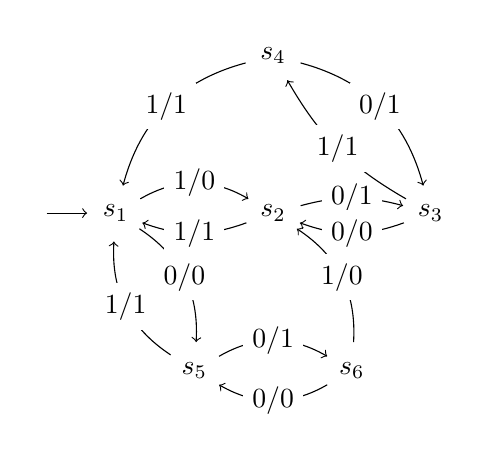
\begin{tikzpicture}[main/.style = {draw, circle}]
          \node[main, draw=none, fill=white](1) at (0,0) {$s_1$};
          \node[left of=1, draw=none](s){};

          \node[main, draw=none, fill=white](2) at (2,0) {$s_2$};
          \node[main, draw=none, fill=white](3) at (4,0) {$s_3$};
          \node[main, draw=none, fill=white](4) at (2,2) {$s_4$};
          \node[main, draw=none, fill=white](5) at (1,-2) {$s_5$};
          \node[main, draw=none, fill=white](6) at (3,-2) {$s_6$};

          \draw[->] (s) to (1);
          \draw[->] (1) to [bend left = 30] node[midway, fill=white] {1/0} (2);
          \draw[->] (1) to [bend left = 30] node[midway, fill=white] {0/0} (5);
          \draw[->] (2) to [bend left = 20] node[midway, fill=white] {1/1} (1);
          \draw[->] (2) to [bend left = 15] node[midway, fill=white] {0/1} (3);
          \draw[->] (3) to [bend left = 15] node[midway, fill=white] {1/1} (4);
          \draw[->] (3) to [bend left = 20] node[midway, fill=white] {0/0} (2);
          \draw[->] (4) to [bend right = 30] node[midway, fill=white] {1/1} (1);
          \draw[->] (4) to [bend left = 30] node[midway, fill=white] {0/1} (3);
          \draw[->] (5) to [bend left = 30] node[midway, fill=white] {1/1} (1);
          \draw[->] (5) to [bend left = 30] node[midway, fill=white] {0/1} (6);
          \draw[->] (6) to [bend right = 30] node[midway, fill=white] {1/0} (2);
          \draw[->] (6) to [bend left = 30] node[midway, fill=white] {0/0} (5);
        \end{tikzpicture}
      \end{exercisenoinc}
    \end{frame}

    \begin{frame}{Aufgabe \thesection}{Reduktion von Mealy Automaten, Schaltwerke}
      \begin{solutionnoinc}
        % Äquivalente Zustände: Bei gleicher Eingabe - gleiche Ausgabe und gleicher Folgezustand\\
        \centering
        \begin{tikzpicture}[main/.style = {draw, circle}]
            \node[main, fill=SecondaryColorDimmed, draw=none](1) at (0,0) {$s_1$};
            \node[left of=1, draw=none](s){};

            \node[main, fill=PrimaryColorDimmed, draw=none](2) at (2,0) {$s_2$};
            \node[main, draw=none, fill=white](3) at (4,0) {$s_3$};
            \node[main, fill=PrimaryColorDimmed, draw=none](4) at (2,2) {$s_4$};
            \node[main, draw=none, fill=white](5) at (1,-2) {$s_5$};
            \node[main, fill=SecondaryColorDimmed, draw=none](6) at (3,-2) {$s_6$};

            \draw[->] (s) to (1);
            \draw[->] (1) to [bend left = 30] node[midway, fill=SecondaryColorDimmed, rounded corners=5pt] {1/0} (2);
            \draw[->] (2) to [bend left = 20] node[midway, fill= PrimaryColorDimmed, rounded corners=5pt] {1/1} (1);
            \draw[->] (3) to [bend left = 15] node[midway, fill= white] {1/1} (4);
            \draw[->] (3) to [bend left = 20] node[midway, fill= white] {0/0} (2);
            \draw[->] (4) to [bend right = 30] node[midway, fill= PrimaryColorDimmed, rounded corners=5pt] {1/1} (1);
            \draw[->] (4) to [bend left = 30] node[midway, fill= PrimaryColorDimmed, rounded corners=5pt] {0/1} (3);
            \draw[->] (5) to [bend left = 30] node[midway, fill= white] {1/1} (1);
            \draw[->] (5) to [bend left = 30] node[midway, fill= white] {0/1} (6);
            \draw[->] (6) to [bend right = 30] node[midway, fill=SecondaryColorDimmed, rounded corners=5pt] {1/0} (2);
            \draw[->] (6) to [bend left = 30] node[midway, fill=SecondaryColorDimmed, rounded corners=5pt] {0/0} (5);
            \draw[->] (1) to [bend left = 30] node[midway, fill=SecondaryColorDimmed, rounded corners=5pt] {0/0} (5);
            \draw[->] (2) to [bend left = 15] node[midway, fill= PrimaryColorDimmed, rounded corners=5pt] {0/1} (3);
            \end{tikzpicture}
      \end{solutionnoinc}
    \end{frame}

    \begin{frame}{Aufgabe \thesection}{Reduktion von Mealy Automaten, Schaltwerke}
      \begin{solution}
        \centering
        \begin{tikzpicture}[main/.style = {draw, circle}]
          \node[main, fill=SecondaryColorDimmed, draw=none](1) at (0,0) {$s_{1/6}$};
          \node[left of=1, draw=none](s){};

          \node[main, fill=PrimaryColorDimmed, draw=none](2) at (3,0) {$s_{2/4}$};
          \node[main, draw=none, fill=white](3) at (6,0) {$s_3$};
          \node[main, draw=none, fill=white](5) at (0,-3) {$s_5$};

          \draw[->] (s) to (1);
          \draw[->] (1) to [bend left = 20] node[midway, fill= SecondaryColorDimmed] {1/0} (2);
          \draw[->] (1) to [bend left = 60] node[midway, fill=SecondaryColorDimmed] {0/0} (5);
          \draw[->] (2) to [bend left = 20] node[midway, fill=PrimaryColorDimmed] {1/1} (1);
          \draw[->] (2) to [bend left = 35] node[midway, fill=PrimaryColorDimmed] {0/1} (3);
          \draw[->] (3) to node[midway, fill= white] {1/1} (2);
          \draw[->] (3) to [bend left = 35] node[midway, fill= white] {0/0} (2);
          \draw[->] (5) to [bend left = 60] node[midway, fill= white] {1/1} (1);
          \draw[->] (5) to node[midway, fill= white] {0/1} (1);
        \end{tikzpicture}
      \end{solution}
    \end{frame}

    \begin{frame}{Aufgabe \thesection}{Reduktion von Mealy Automaten, Schaltwerke}
        \begin{block}{Lösung}
          \begin{itemize}
            \item $s_{i} = (z_1, z_0), s_{1,6} = (0, 0), s_{2,4} = (0, 1), s_{3} = (1, 0), s_{5} = (1, 1)$
          \end{itemize}
          \includegraphics[height=0.5\paperheight, center]{./figures/Mealy-reduziert-Übergangstafel.png}
        \end{block}
    \end{frame}

    \begin{frame}{Aufgabe \thesection}{Reduktion von Mealy Automaten, Schaltwerke}
      % \begin{exercisenoinc}
      %   \includegraphics[height=0.5\paperheight, center]{./figures/Mealy-reduziert-Übergangstafel-Funktionen.png}
      % \end{exercisenoinc}
      \begin{solution}
        \begin{itemize}
          \item $z_0^{t+1} = \overline{x}\overline{z_1^t}\overline{z_0^t} +  x\overline{z_1^t}\overline{z_0^t} + \overline{x}z_1^t\overline{z_0^t} + xz_1^t\overline{z_0^t} \overset{Red.}{=} \overline{z}_0^t$
          \item $z_1^{t+1} = \overline{x}\overline{z_1^t}\overline{z_0^t} + \overline{x}\overline{z_1^t}z_0^t \overset{Red.}{=} \overline{x + z_1^t} = \overline{x} \cdot \overline{z}_1^t$
          \item $y         = \overline{x}\overline{z_1^t}z_0^t + x\overline{z_1^t}z_0^t + xz_1^t\overline{z_0^t} + \overline{x}z_1^tz_0^t + xz_1^tz_0^t \overset{Red.}{=} z_0^t + x \cdot z_1^t$
        \end{itemize}
        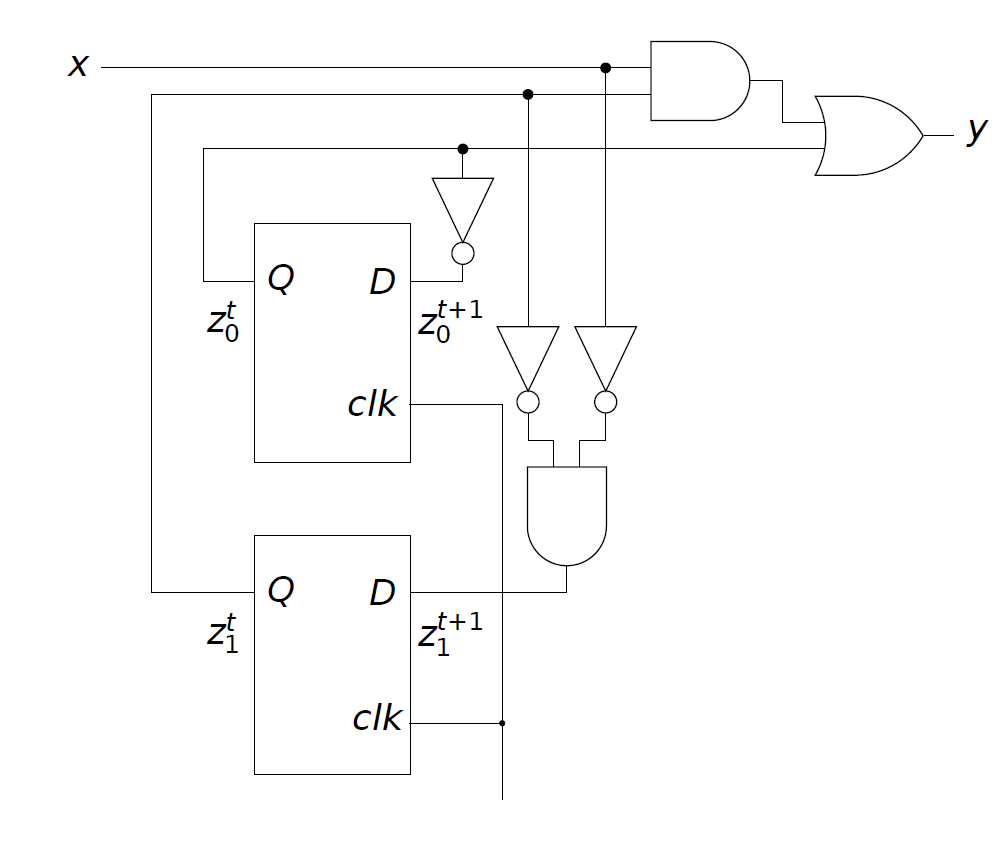
\includegraphics[height=0.5\paperheight, center]{./figures/Mealy-reduziert-Schaltwerk.png}
      \end{solution}
    \end{frame}
